% !TEX root =  CurvedFoldedDogs.tex

\section{Optimization} \label{sec:implementation}
We employ \theoremref{Thm:supporting_plane} and its discretization in \equref{eq:folding_const} in a simple algorithm to enforce folding along crease curves while deforming piecewise DOGs. The algorithm aims to minimize an objective function while keeping the DOG constraints and ensuring the formation of folds along all crease curves.

\subsection{Problem setup}
We model our curved folded surfaces as a quad mesh, with a separate connected component for each patch. We denote the set of $n$ mesh vertices in $\R^3$ by $V$, the vertex positions (variables) by $\x \in \R^{3n}$, and the quad mesh faces by $F$. Each connected component is a DOG, i.e., it has the connectivity of a subset of $\Z^2$ and satisfies the DOG angle constraints \cite{rabi18}, which we denote as $\phi_{d_i}(\x) = 0, 1 \leq i \leq m$.

We are interested in deformations that fold the surface along all crease curves in a given crease pattern using \theoremref{Thm:supporting_plane} and enforcing \equref{eq:folding_const}. We enforce these constraints on all crease points, which are points on crease curves that are not crease vertices, with the exception of crease points that have the following degeneracies on the flattened mesh (see \figref{fig:fold_const_degeneracies}):
\begin{enumerate}
	\item degenerate osculating plane: crease points with a curvature smaller than a threshold $\kappa_\eps$; \label{item:deg_osc}
	\item degenerate edge: crease points on an edge, splitting it into two parts where one is shorter than $\eps_{r}$\% of the other; \label{item:deg_edge}
	\item degenerate angle with the intersecting DOG tangent: crease points where the tangent directions $t_1,t_2$ form an angle with one of the edges $e_f,e_b$ that is smaller than $\eps_\alpha$. \label{item:deg_tan_angle}
\end{enumerate}
We use the constants $\kappa_\epsilon=\text{1e-5}, \eps_r=5\%, \eps_\alpha=3^{\circ}$. We denote the folding constraints by $\phi_{f_j}(\x) = 0, 1 \leq f_j \leq n_f$.

\begin{figure} [h]
	\centering
	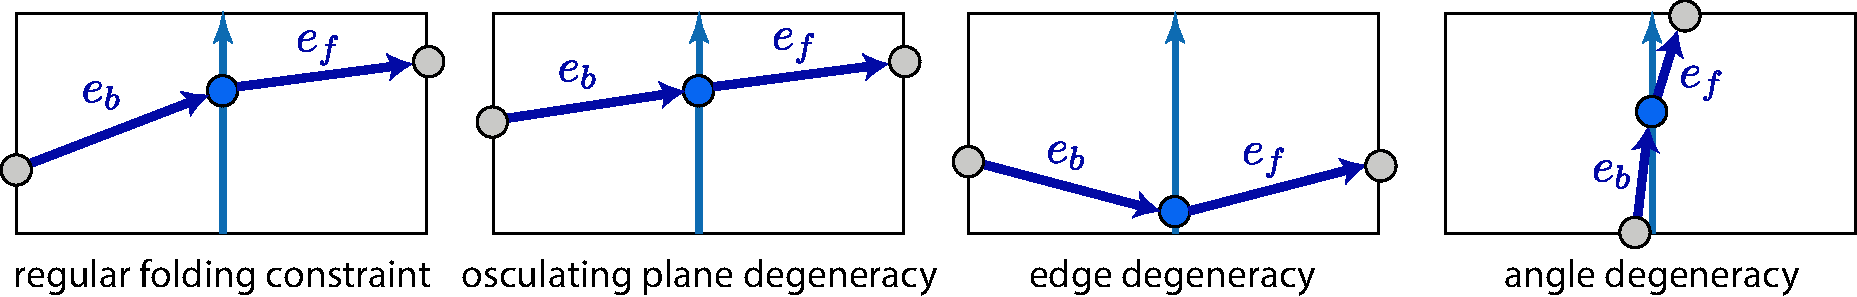
\includegraphics[width=\linewidth]{figures/fold_const_degeneracies}
	\caption{A folding edge constraint defined on a blue crease point splitting the blue edge and degenerate cases where we do not enforce the constraint. From left to right: A regular folding edge constraint, instabilities in the osculating plane's normal as $\frac{e_b \times e_f}{\|e_b \times e_f\|}$ caused by $e_b,e_f$ being almost collinear, degenerate edges as one part of the edge split by the blue crease point is comparably very short, and lastly a very small angle between $e_b$ and the DOG edge crossing the blue point. An angle degeneracy often occurs before or after an edge degeneracy.}
	\label{fig:fold_const_degeneracies}
\end{figure}

The problems we solve in this paper can be written in the form:
\begin{equation} \label{eq:const_opt}
\begin{aligned}
& \argmin_x f(x) \\
& \textrm{subject to} \\
& \phi_{d_i}(\x) = 0, \ \  i = 1, \ldots, m, \\
& \phi_{f_j}(\x) = 0, \ \  j = 1, \ldots, n_f, \\ 
\end{aligned}
\end{equation}
where $f$ is an objective function composed of a weighted sum of a bending objective, isometry objective, positional constraints and other terms as specified in \secref{sec:dog_obj}.

\subsection{Folding constraints}
Motivated by the fact that in the smooth case, one cannot move from a folded to a non-folded configuration around a non-planar point, we strive to always satisfy $\phi_{f_j}(x) = 0$ exactly. The common starting point of a flat surface is an interesting case, as it is a bifurcation point between surfaces satisfying \theoremref{Thm:supporting_plane} and those that do not, which also holds for the discretization \equref{eq:folding_const_normalized}. To that end, we solve our problem with an iterative sequential quadratic programming (SQP) solver with a line search, complemented with two simple strategies to handle the folding constraints $\phi_{f_i}(\x)$:
\begin{enumerate}
	\item a penalty term \cite{nocedal} punishing  deviation from the constraints; \label{opt:penalty}
	\item a line search method that backtracks if the resulting mesh does not exactly satisfy $\phi_{f_j}(\x) = 0, i = 1,...,n_f$.
\end{enumerate}
Since the functions $\text{sgn}(x),H(x)$ involved in the constraints $\phi_{d_i}(\x)$ are not $C^1$, we replace them by the approximations:
%
\begin{align} 
\begin{split}\label{eq:const_inner}
&\text{sgn}(x) \approx \tanh(hx) \\
&H(x) \approx  \left\{\begin{array}{@{}l@{\thinspace}l}
0  &: \text{if } x \leq 0, \\
\frac{x^2}{x^2+\delta} &: \text{if } x = 0, \delta > 0 \\
\end{array}\right.
\end{split}
\end{align}
using the fixed parameters $h=1000,\delta = \text{1e-5}$. Our approximation for $H(x)$ is taken from \cite{l0_approximation,autocuts}.  The use in a homotopy based optimization necessitates an approximation for $H(x)$ that vanishes on a flat mesh, and therefore we do not use the common approximation for the Heaviside function $H(x) \approx \hat{H}(x) =  \frac{1+\tanh(hx)}{2}$ because $\hat H(0) = \frac{1}{2}$.

We refer to the approximated constraints as $\phi^*_{f_j}(\x)$ and replace the optimization problem \eqref{eq:const_opt} with the following problem:
\begin{equation} \label{eq:const_opt_penalty}
\begin{aligned}
& \argmin_x f(x) + \omega \sum \|\phi^*_{f_j}(\x)\|_2^2 \\
& \textrm{subject to} \\
& \phi_{d_i}(\x) = 0, \ \  i = 1, \ldots, m. \\ 
\end{aligned}
\end{equation}
Here, $\omega > 0$ is a metaparameter initialized as $\omega_0 = 1$, which doubles its value if the line search cannot find a point satisfying the supporting plane conditions exactly. In practice, the penalty term only affects points that are very close to being planar, while approaching zero very quickly around already folded points.

\subsection{Equality constrained SQP}
For ease of notation, we use the following to refer to the objective of \equref{eq:const_opt_penalty}:
\begin{equation}
f_\omega(\x) = f(x) + \omega \sum \|\phi^*_{f_j}(\x)\|_2^2.
\end{equation}
We minimize \eqref{eq:const_opt_penalty} using SQP with a line search \cite{nocedal}. Given a set of variables at a given iteration $x^k$ and current values of Lagrange multipliers $\lambda^k$, a line search equality constrained SQP algorithm iteratively finds the next direction for a line search of \equref{eq:const_opt_penalty}, by which it sets the next variables $x^{k+1}$ by solving a KKT system of the form:
%
\begin{equation} \label{eq:KKT_eps}
\begin{aligned}
&{K} \begin{pmatrix} d^{k+1} \\ \lambda^{k+1} \end{pmatrix}=\mathbf{b}, \ \text{where} \\
&{K}=\begin{pmatrix}
{\Delta^2_{xx}\mathcal{L}(x^k,\lambda^k)} & {J^\tr}(\x^k)\\
{J(\x^k)} &  0 \\
\end{pmatrix}, \ \ 
\mathbf{b}=\begin{pmatrix}
{\nabla f_\omega(x^k)} \\ 
-\phi_{d_i}(x^k)\\
\end{pmatrix},
\end{aligned}
\end{equation}
%
where $J(\x)$ is the Jacobian of the equality constraints in \equref{eq:const_opt_penalty}, $\Delta^2_{xx}\mathcal{L}(x,\lambda) = H_{f_\omega}(x)+\sum\lambda_i^{k} \nabla \phi_{d_i}(x)$ is the Lagrangian of the problem and $H_{f_\omega}(\x)$ is the Hessian of $f_\omega(\x)$.

Following \cite{rabi2018shape}, we use a minimally modified Jacobian $J^*(x)$ to deal with singularities in DOGs. We also replace the Hessian of the objective $H_{f_\omega}(\x)$ by a convex approximation, which we denote by $H^*_{f_\omega}(\x)$, as detailed in \secref{sec:dog_obj}, and thus replace the system \eqref{eq:KKT_eps} by:
%
\begin{align} 
\label{eq:KKT_us}
&{K} \begin{pmatrix} d^{k+1} \\ \lambda^{k+1} \end{pmatrix}=\mathbf{b}, \ \text{where} \\
\nonumber
&{K}=\begin{pmatrix}
{ H^*_{f_\omega}(\x^k)+\sum\lambda_i^{k} \nabla \phi_{d_i}(\x^k)} & {J^{*^\tr}(\x^k)}\\
{J^*(\x^k)} &  0 \\
\end{pmatrix}, \ \ 
\mathbf{b}=\begin{pmatrix}
{\nabla f_\omega(x^k)} \\ 
-\phi_{d_i}(x^k)\\
\end{pmatrix}.
\end{align}

We note that in \cite{rabi2018shape} the authors discretize Laplacian metric flows by solving a similar system with a Laplacian instead of the objective's Lagrangian. However, we found that replacing the Laplacian by the Lagrangian followed by convexifying the Hessian performs significantly better, especially on larger models. As common in SQP algorithms, we use a merit function to guide our line search, defined as a combination of the objective and the constraints. The line search chooses step sizes that reduce the objective and keep the DOG angle constraints numerically feasible, while backtracking if a point does not satisfy the folding constraints exactly.

This removes the need for the slower LBFGS constraints' projection used by \cite{rabi18,rabi2018shape}. We use the $L_2$ merit function \cite{nocedal}:
\begin{equation}
\psi(\x;\mu) = f_\omega(\x)+\mu\sum\|\phi_{d_i}(x)\|_2,
\end{equation}
where we update the parameter $\mu^k$ at each iteration using the absolute values of the Lagrange multipliers \cite{nocedal}:
\begin{equation}
\mu^k = \max\{c_\mu \cdot \max\{|{\lambda_i^k}|\},\ \mu_0\},
\end{equation}
with $c_\mu = 1.1$ and $\mu_0 = 0.05$.

\subsection{Objectives and constraints} \label{sec:dog_obj}
Our objective $f$ is composed of a weighted sum of various functions measuring bending, stretch, positional constraints and dihedral angles.
We use an integrated squared mean curvature bending objective taken from \cite{rabi2018shape}, and we exploit the fact that it is quadratic and convex under isometric deformations (\cite{quadratic_bending}):
\begin{equation}
f_\text{H}(\x) = 0.5\x^t(L^tM^{-1}L)\x,
\end{equation}
where $L$ is the DOG Laplacian and $M$ is a diagonal mass matrix defined by the DOG vertex area \cite{rabi2018shape}.

 We employ \lemmaref{lem:tangents_dihedral} to constrain the folding angle at a given crease point using the constraint
\begin{equation}
\phi_{\text{d}_{c^i}}(\x) := \langle t_1^i, t_2^i \rangle - \cos^2(\alpha^i) - \sin^2(\alpha^i) \cos(\theta^i) = 0,
\end{equation}
where $c^i$ is the index of the crease point along the edge defined as a linear combination of two vertices, $t_1^i$, $t_2^i$, $\alpha^i$ are as defined in \secref{sec:folding_angle} and \figref{fig:fold_angle_and_tangent_angles}, and $\theta^i$ is the desired dihedral angle at the crease point $c^i$. Under isometry $t_1^i,t_2^i$ are linear in the net vertex locations, $\alpha^i$ is fixed, and the constraint is quadratic.

Let $e$ be an edge on the net mesh, $l_e$ its length and $l_e^0$ the length in the reference net mesh. We define the following quadratic isometry constraints:
\begin{equation}
\phi_\text{iso}(\x)_e := l_e^2 - {l_e^0}^2 = 0.
\end{equation}
We maintain continuity along the patches with a set of linear equality constraints on duplicated crease points \cite{rabi2018shape}, which we denote by $\phi_\text{cont}(\x) = 0$. Lastly, we allow the user to specify positional constraints on vertices or crease edge points, including constraints requiring two points to have the same coordinate (\MiR{point to teaser or sphere figure}, denoting this user defined set of constraints by $\phi_{\text{pos}}(\x) = 0$.
We enforce the dihedral, positional, isometry and patches continuity constraints in a soft manner by using a penalty on their squared deviation, denoted accordingly by $f_\text{D}(\x), f_\text{pos}(\x), f_\text{iso}(\x), f_\text{cont}(\x)$. These sum of squares objectives are not convex, and we replace their Hessian in our optimization with their Gauss-Newton's Hessian approximation. We do the same for $\sum \|\phi^*_{f_i}(\x)\|_2^2$. Isometry is enforced as a soft constraint $f_\text{iso}(\x)$, as advised by the degrees of freedom analysis in \cite{rabi18,rabi2018shape}, but we emphasize that all our results have an average relative edge stretch that is less than $0.003$, and a maximum stretch below $4$, where our surfaces are normalized to have an average edge length of $1$. As opposed to \cite{rabi2018shape}, we also encode  $\phi_\text{cont}(\x)$  as a soft constraint, as we have noticed a significant improvement in the quality and smoothness of crease patterns when these are enforced as a soft penalty with a large weight,
%\MiR{ok to say?, this is mostly important in the curved constrained case for interactivity, as if we run the interpolation much slower then we can still use hard constraints},  
and our results have an average continuity deviation of $0.0002$ and a maximum of $0.0035$. We note that the constrained shape space analysis in \cite{rabi2018shape} only concerns the DOG angle constraints, and complicated crease patterns give rise to a large set of additional linear constraints.
 
The objective we optimize is then:
\begin{equation}
f(\x) = w_Hf_\text{H}+w_{pos}f_\text{pos}+w_Df_\text{D}+w_{iso}f_\text{iso}+w_{cont}f_\text{cont}
\end{equation}
Throughout the paper, unless stated otherwise, we use $w_H = 1$, $w_\text{pos}=5$,$w_D = 100$, $w_\text{iso}= \frac{20000}{\|E\|}$, $w_{cont} = 1e4$, where $\|E\|$ is the number of edges in the net mesh (i.e., for a mesh with $1000$ vertices $w_\text{iso}=20$). Our meshes are always scaled to have an average edge length of $1$ and therefore using a different resolution for the same geometry keeps our bending objective the same, but scales the isometric objective by the number of edges.